\documentclass[listings]{labreport}
\usepackage{amsmath}
\usepackage{multirow}
\usepackage{multicol}
\subject{Методы оптимизации}
\titleparts{Расчетная работа №2}{Вариант 8}
\students{Лабушев Тимофей}

\begin{document}

\maketitlepage

\section*{Условие задачи}

Дана транспортная сеть, состоящая из 7 вершин, связи между которыми
заданы с помощью матрицы инцидентности. Найти оптимальный грузопоток.

\[
  G = 
\begin{pmatrix}
  0 & 1 & 0 & 0 & 1 & 0 & 0 \\
  0 & 0 & 1 & 1 & 0 & 0 & 1 \\
  0 & 0 & 0 & 1 & 0 & 1 & 0 \\
  0 & 0 & 0 & 0 & 1 & 0 & 1 \\
  0 & 0 & 0 & 0 & 0 & 1 & 0 \\
  0 & 0 & 0 & 0 & 0 & 0 & 1 \\
  0 & 0 & 0 & 0 & 0 & 0 & 0
\end{pmatrix}
\]

Интенсивности источников и потребителей:

$$d_1 = 17,\ d_2 = 19,\ d_3 = d_4 = 0,\ d_5 = -8,\ d_6 = -12,\ d_7 = -16$$ 
$$r_{15} = 4,\ r_{27} = 4$$

Матрица промежуточных расходов:

\[
  C =
\begin{pmatrix}
0 & 1 & 0 & 0 & 1 & 0 & 0 \\
0 & 0 & 2 & 3 & 0 & 0 & 6 \\
0 & 0 & 0 & 7 & 0 & 9 & 0 \\
0 & 0 & 0 & 0 & 10 & 0 & 10 \\
0 & 0 & 0 & 0 & 0 & 9 & 0 \\
0 & 0 & 0 & 0 & 0 & 0 & 4 \\
0 & 0 & 0 & 0 & 0 & 0 & 0
\end{pmatrix}
\]

Сеть с ограничениями:

\begin{multicols}{2}

\begin{tabular}{|c|c|c|c|c|}
\hline
$i$ & $d_i$ & $(i,j)$ & $C_{ij}$ & $r_{ij}$ \\ \hline
\multirow{2}{*}{1} & \multirow{2}{*}{11} & (1,2) & 1 & - \\
& & (1,5) & 1 & 4 \\ \hline
\multirow{3}{*}{2} & \multirow{3}{*}{19} & (2,3) & 2 & - \\
& & (2,4) & 3 & - \\
& & (2,7) & 6 & 4 \\ \hline
\multirow{2}{*}{3} & \multirow{2}{*}{0} & (3,4) & 7 & - \\
& & (3,6) & 9 & - \\ \hline
\multirow{2}{*}{4} & \multirow{2}{*}{0} & (4,5) & 10 & - \\
& & (4,7) & 10 & - \\ \hline
5 & -8 & (5,6) & 9 & - \\ \hline
6 & -12 & (6,7) & 4 & - \\ \hline
7 & -16 & - & - & - \\ \hline
\end{tabular}

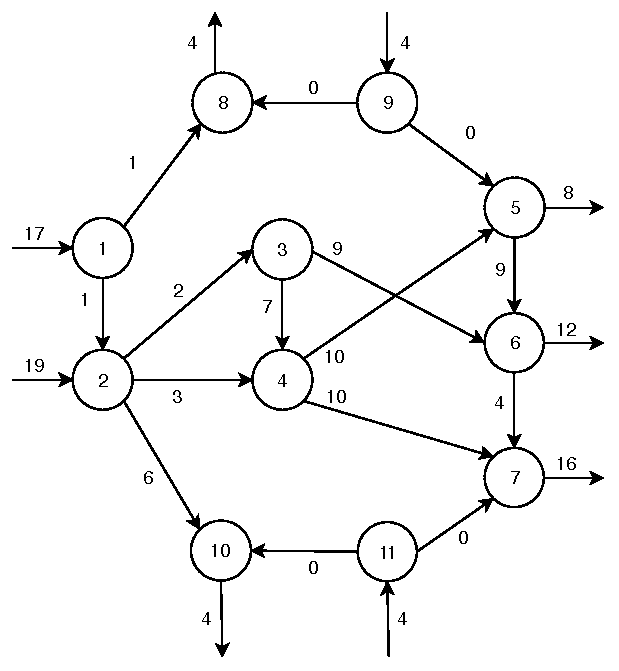
\includegraphics[width=0.45\textwidth]{graph1.pdf}
\end{multicols}

\section*{Решение}

Найдем кратчайшие пути:

\begin{multicols}{2}
\begin{tabular}{|c|c|c|}
\cline{1-2}
(1,2): 1 & (1,8): 1 \\ \hline
(2,3): 3 & (2,4): 4 & (2,10): 7 \\ \hline
(3,4): 10 & (3,6): 12 \\ \cline{1-2}
(4,5): 14 & (4,7): 14 \\ \cline{1-2}
(5,6): 23 \\ \cline{1-1}
(6,7): 27 \\ \cline{1-1}
\end{tabular}

\noindent
1-5: 1,2,4,5 (14) \\
1-6: 1,2,3,6 (12) \\
1-7: 1,2,4,7 (14) \\
1-8: 1,8 (1) \\
1-10: 1,2,10 (7) \\
\end{multicols}

\begin{multicols}{2}
\begin{tabular}{|c|c|c|}
\hline
(2,3): 2 & (2,4): 3 & (2,10): 6 \\ \hline
(3,4): 9 & (3,6): 11 \\ \cline{1-2}
(4,5): 13 & (4,7): 13 \\ \cline{1-2}
(5,6): 22 \\ \cline{1-1}
(6,7): 17 \\ \cline{1-1}
\end{tabular}

\noindent
2-5: 2,4,5 (13) \\
2-6: 2,3,6 (11) \\
2-7: 2,4,7 (13) \\
2-8: - \\
2-10: 2,10 (6) \\
\end{multicols}

\begin{multicols}{2}
\begin{tabular}{|c|c|}
\hline
(9,5): 0 & (9,8): 0 \\ \hline
(5,6): 9 \\ \cline{1-1}
(6,7): 13 \\ \cline{1-1}
\end{tabular}

\columnbreak 
\noindent
9-5: 9,5 (0) \\
9-6: 9,5,6 (9) \\
9-7: 9,5,6,7 (13) \\
9-8: 9,8 (0) \\
9-10: - \\
\end{multicols}

\begin{multicols}{2}
\begin{tabular}{|c|}
\hline
(11,7): 0 \\ \hline
(11,10): 0 \\ \hline
\end{tabular}

\columnbreak
\noindent
11-5: - \\
11-6: - \\
11-7: 11,7 (0) \\
11-8: - \\
11-10: 11,10 (0) \\
\end{multicols}

Построим опорный план:

{\renewcommand{\arraystretch}{1.4}
\begin{tabular}{c|c|c|c|c|c|ccccccc}
\multicolumn{1}{c}{} &
  \multicolumn{1}{c}{5} &
  \multicolumn{1}{c}{6} &
  \multicolumn{1}{c}{7} &
  \multicolumn{1}{c}{8} &
  \multicolumn{1}{c}{10} \\ \cline{2-6}
1 & 14 \textsubscript{1} & 12 & 14 \textsubscript{12} & 1 \textsubscript{4} & 7
  & \textit{17}
  & \textbf{\textit{17}}
  & \textit{13}
  & \textit{13}
  & \textbf{\textit{13}}
  & \textit{0}
  \\ \cline{2-6}
2 & 13 \textsubscript{3} & 11 \textsubscript{12} & 13 & - & 6 \textsubscript{4}
  & \textit{19}
  & \textit{19}
  & \textbf{\textit{19}}
  & \textbf{\textit{15}}
  & \textit{0}
  \\ \cline{2-6}
9 & 0 \textsubscript{4} & 9 & 13 & 0 & -
  & \textbf{\textit{4}}
  & \textit{0}
  \\ \cline{2-6}
11 & - & - & 0 \textsubscript{4} & - & 0
  & \textbf{\textit{4}}
  & \textit{0}
  \\ \cline{2-6}
\multicolumn{1}{c}{} &
  \multicolumn{1}{c}{\textbf{\textit{8}}} &
  \multicolumn{1}{c}{\textit{12}} &
  \multicolumn{1}{c}{\textbf{\textit{16}}} &
  \multicolumn{1}{c}{\textit{4}} &
  \multicolumn{1}{c}{\textit{4}} \\
\multicolumn{1}{c}{} &
  \multicolumn{1}{c}{\textit{4}} &
  \multicolumn{1}{c}{\textit{12}} &
  \multicolumn{1}{c}{\textit{12}} &
  \multicolumn{1}{c}{\textbf{\textit{4}}} &
  \multicolumn{1}{c}{\textit{4}} \\
\multicolumn{1}{c}{} &
  \multicolumn{1}{c}{\textit{4}} &
  \multicolumn{1}{c}{\textit{12}} &
  \multicolumn{1}{c}{\textit{12}} &
  \multicolumn{1}{c}{\textit{0}} &
  \multicolumn{1}{c}{\textbf{\textit{4}}} \\
\multicolumn{1}{c}{} &
  \multicolumn{1}{c}{\textbf{\textit{4}}} &
  \multicolumn{1}{c}{\textbf{\textit{12}}} &
  \multicolumn{1}{c}{\textit{12}} &
  \multicolumn{1}{c}{} &
  \multicolumn{1}{c}{\textit{0}} \\
\multicolumn{1}{c}{} &
  \multicolumn{1}{c}{\textbf{\textit{1}}} &
  \multicolumn{1}{c}{\textit{0}} &
  \multicolumn{1}{c}{\textbf{\textit{12}}} &
  \multicolumn{1}{c}{} &
  \multicolumn{1}{c}{} \\
\multicolumn{1}{c}{} &
  \multicolumn{1}{c}{\textit{0}} &
  \multicolumn{1}{c}{} &
  \multicolumn{1}{c}{\textit{0}} &
  \multicolumn{1}{c}{} &
  \multicolumn{1}{c}{} \\
\end{tabular}}

Полученный базис:

\begin{tabular}{c|c|c|c|c|c|}
\multicolumn{1}{c}{} &
  \multicolumn{1}{c}{v1} &
  \multicolumn{1}{c}{v2} &
  \multicolumn{1}{c}{v3} &
  \multicolumn{1}{c}{v4} &
  \multicolumn{1}{c}{v5} \\ \cline{2-6}
u1 & 1 & & 12 & 4 & \\ \cline{2-6}
u2 & 3 & 12 & & & 4 \\ \cline{2-6}
u3 & 4 & & & & \\ \cline{2-6}
u4 & & & 4 & & \\ \cline{2-6}
\end{tabular}\\[2mm]

Проверим оптимальность полученного опорного плана:

$$
\begin{cases}
  u_1 + v_1 = 14 \\
  u_2 + v_1 = 13 \\
  u_2 + v_2 = 11 \\
  u_2 + v_5 = 6 \\
  u_3 + v_1 = 0 \\
  u_1 + v_3 = 14 \\
  u_4 + v_3 = 0 \\
  u_1 + v_4 = 1
\end{cases}
\implies
\begin{cases}
  u_1 = 0 \\
  u_2 = -1 \\
  u_3 = -14 \\
  u_4 = -14 \\
  v_1 = 14 \\
  v_2 = 12 \\
  v_3 = 14 \\
  v_4 = 1 \\
  v_5 = 7
\end{cases}
$$

{\renewcommand{\arraystretch}{1.4}
\begin{tabular}{c|c|c|c|c|c|c}
\multicolumn{1}{c}{} &
  \multicolumn{1}{c}{5} &
  \multicolumn{1}{c}{6} &
  \multicolumn{1}{c}{7} &
  \multicolumn{1}{c}{8} &
  \multicolumn{1}{c}{10} &
  \multicolumn{1}{c}{u} \\ \cline{2-6}
1 & 14 & 12 \textsubscript{0} & 14 & 1 & 7 \textsubscript{0} & 0 \\ \cline{2-6}
2 & 13 & 11 & 13 \textsubscript{0} & - & 6 & -1 \\ \cline{2-6}
3 & 0 & 9 \textsubscript{-11} & 13 \textsubscript{-13} & 0 \textsubscript{-13} & - & -14 \\ \cline{2-6}
4 & - & - & 0 & - & 0 \textsubscript{-7} & -14 \\ \cline{2-6}
\multicolumn{1}{c}{v} &
  \multicolumn{1}{c}{14} &
  \multicolumn{1}{c}{12} &
  \multicolumn{1}{c}{14} &
  \multicolumn{1}{c}{1} &
  \multicolumn{1}{c}{7} \\
\end{tabular}}

Опорный план является оптимальным ($u_{ij} + v_{ij} - C_{ij} \leqslant 0,\ i = \overline{1,4},\ j = \overline{1,5}$).

$$F = 1\cdot14 + 12\cdot14 + 4\cdot1 + 3\cdot13 + 12\cdot11 + 4\cdot6 + 4\cdot0 + 4\cdot0 = 381$$

\newpage

Найдем оптимальный грузопоток:

\begin{multicols}{2}

\noindent
1-5: 1,2,4,5 (1) \\
1-7: 1,2,4,7 (12) \\
1-8: 1,8 (4) \\
2-5: 2,4,5 (3) \\
2-6: 2,3,6 (12) \\
2-10: 2,10 (4) \\
9-5: 9,5 (4) \\
11-7: 11,7 (4) \\

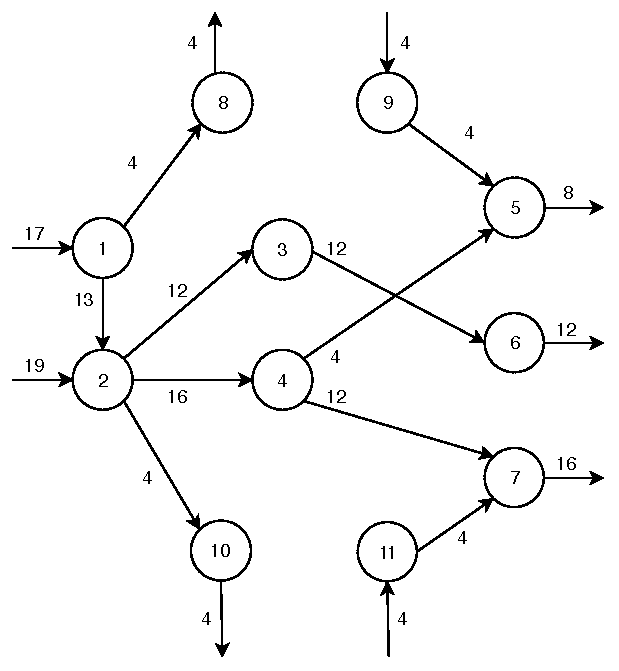
\includegraphics[width=0.45\textwidth]{graph2.pdf}
\end{multicols}

\section*{Ответ}

$F = 381$\\

Оптимальный грузопоток:

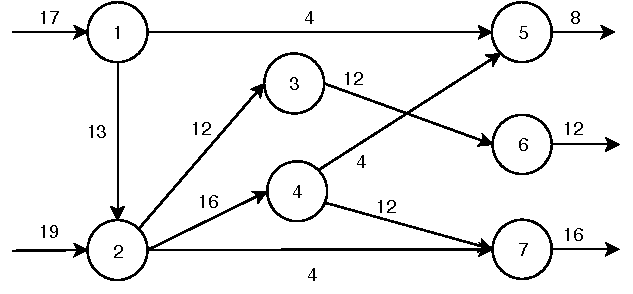
\includegraphics[width=0.6\textwidth]{graph3.pdf}

\end{document}
